\chapter{0次ホールド}
    \providecommand{\FT}[1]{\mathcal{F}\parens*{#1}}
    \providecommand{\Ts}{T_\text{s}}
    \section{0次ホールドされた離散時間信号の周波数特性}
        \label{0次ホールドされた離散時間信号の周波数特性}
        \newcommand{\xd}{x_\text{d}}
        \newcommand{\Xd}{X_\text{d}}
        \subsection{動機}
            離散時間信号を仮に量子化誤差なくDA変換できた場合の周波数スペクトルを計算したい。
        \subsection{主張}
            $\xd:\integers\to\complexNumbers$ を離散時間信号とする。
            $\Xd$ を $\xd$ のDTFTとする。
            $\Ts>0$ をサンプル周期として $\xd$ の0次ホールドで生成した階段状の連続時間信号を $x$ とする。
            $u:\realNumbers\to\braces{0,1}$ を幅 $\Ts$ のパルスとする。
            \[
                u(t) = \begin{cases}
                    1 & 0\leq t < \Ts \\
                    0 & \text{otherwise}
                \end{cases}
            \]
            $x$ は次式で表される。
            \[ x(t) = \sum_{n=-\infty}^\infty \xd(n)u(t-n\Ts) \]
            次の図は $\Ts=1,\xd(n) = \sin\parens{2\pi n/12}\;(0\leq n\leq 24),\;\xd(n) = 0\;(n<0,24<n)$ の例である。
            \begin{figure}[H]
                \centering
                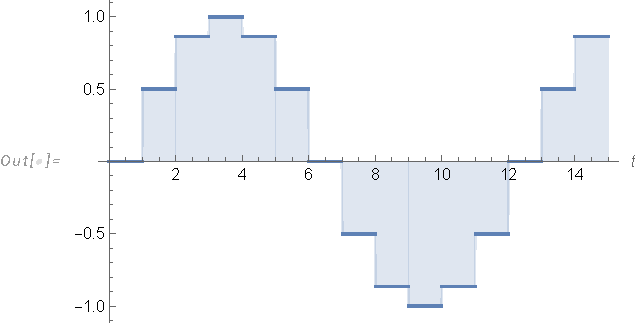
\includegraphics[keepaspectratio, scale=0.8]
                {parts/time-discretization/chapters/up-sampling/imgs/x1.pdf}
                \caption{$x$の例}
                \label{離散時間信号のDAC出力の例}
            \end{figure}
            以上の下、 $x$ のFourier変換 $X$ は次式である。
            \[ X(\omega) = \frac{\Ts}{\sqrt{2\pi}}\exp\parens*{-i\frac{\Ts}{2}\omega}\parens*{\sinc \frac{\Ts}{2}\omega}\Xd(\omega) \]
            $\Xd(\omega)$ が $2\pi/\Ts$ 周期関数であることに注意すれば、$\Xd(\omega)$ の第1 Nyquist領域の形状が位相回転 $\exp\parens{-i \omega n\Ts}$ とレベル減衰 $\sinc\omega\Ts/2$ を伴いつつ周期 $2\pi$ で無限に繰り返されていることがわかる。
            次の図は\ref{離散時間信号のDAC出力の例}に対応する $X$ の例である。
            \begin{figure}[H]
                \centering
                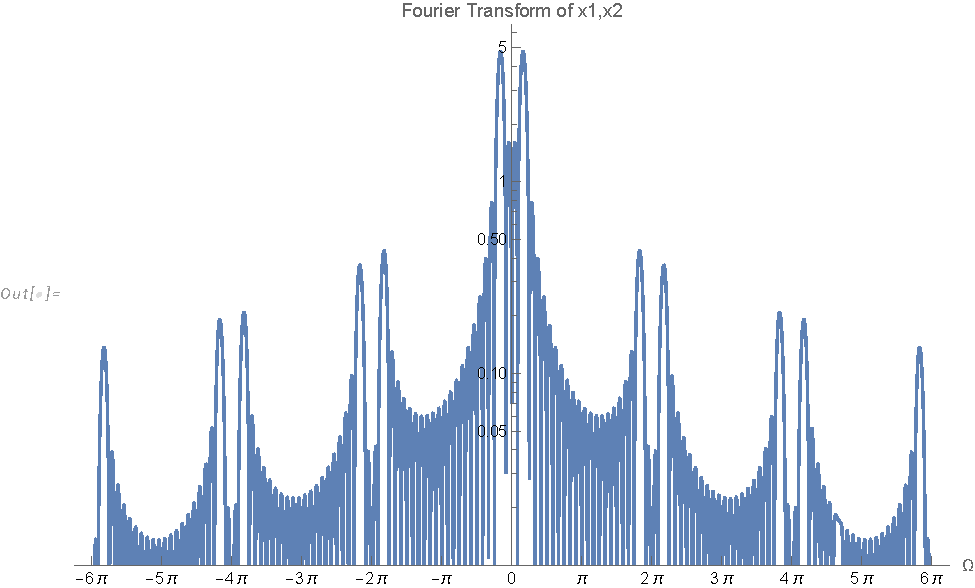
\includegraphics[keepaspectratio, scale=0.8]
                {parts/time-discretization/chapters/up-sampling/imgs/FT_of_x1.pdf}
                \caption{$X$の例。横軸は正規化各周波数}
            \end{figure}
        \subsection{導出}
            \begin{proof}
                \quad\par
                \[ X(\omega) = \FT{\sum_{n=-\infty}^\infty \xd(n)u(t-n\Ts)}(\omega) = \sum_{n=-\infty}^\infty \xd(n)\FT{u(t-n\Ts)}(\omega) \tag{1} \]
                ここで次式が成り立つ。
                \begin{align*}
                    \FT{u(t-n\Ts)}(\omega) &= \exp\parens*{-i \omega n\Ts}\FT{u}(\omega) = \exp\parens*{-i \omega n\Ts}\frac{1}{\sqrt{2\pi}}\integrate{0}{\Ts}{\exp\parens*{-i\omega t}}{}{t} \\
                    &= \frac{i}{\omega\sqrt{2\pi}}\parens*{\exp\parens*{-i \omega\Ts}-1}\exp\parens*{-i \omega n\Ts} \\
                    &= \frac{i}{\omega\sqrt{2\pi}}\exp\parens{-i \omega n\Ts}\exp\parens{-i \omega\Ts/2}\parens*{\exp\parens*{-i \omega\Ts/2} - \exp\parens*{i \omega\Ts/2}} \\
                    &= \frac{i}{\omega\sqrt{2\pi}}\exp\parens{-i \omega n\Ts}\exp\parens{-i \omega\Ts/2}(-2i)\sin\frac{\omega\Ts}{2} \\
                    &= \frac{2}{\omega\sqrt{2\pi}}\exp\parens{-i \omega n\Ts}\exp\parens{-i \omega\Ts/2}\sin\frac{\omega\Ts}{2} \\
                    &= \frac{\Ts}{\sqrt{2\pi}}\exp\parens{-i \omega n\Ts}\exp\parens{-i \omega\Ts/2}\sinc\frac{\omega\Ts}{2}
                \end{align*}
                これを式(1)に適用して次式を得る。
                \begin{align*}
                    X(\omega) &= \sum_{n=-\infty}^\infty \xd(n)\frac{\Ts}{\sqrt{2\pi}}\exp\parens{-i \omega n\Ts}\exp\parens{-i \omega\Ts/2}\sinc\frac{\omega\Ts}{2} \\
                    &= \frac{\Ts}{\sqrt{2\pi}}\exp\parens{-i \omega\Ts/2}\sinc\frac{\omega\Ts}{2} \sum_{n=-\infty}^\infty \xd(n)\exp\parens{-i \omega n\Ts} \\
                    &= \frac{\Ts}{\sqrt{2\pi}}\exp\parens*{-i\frac{\Ts}{2}\omega}\parens*{\sinc \frac{\Ts}{2}\omega}\Xd(\omega)
                \end{align*}
            \end{proof}
    \section{inverse-sinc-filter}
        \subsection{背景}
            離散時間信号をDA変換した結果のFourier変換には次式で表される変化が積の形で含まれることを\ref{0次ホールドされた離散時間信号の周波数特性}で述べた。
            \[ \sinc \frac{\Ts}{2}\omega = \sinc \frac{\Omega}{2} \]
            ここに $\Ts$ はサンプリング周期, $\Omega$ は正規化各周波数である。
            変化の中には上式の他に $\exp\parens*{-i\frac{\Ts}{2}\omega}$ という項も含まれるが、これは一定の群遅延が加わる(線形位相特性)だけであり、実用上無害なので無視する。
            次の図は $\abs{\sinc \frac{\Omega}{2}}$ をプロットしたものである。
            \begin{figure}[H]
                \centering
                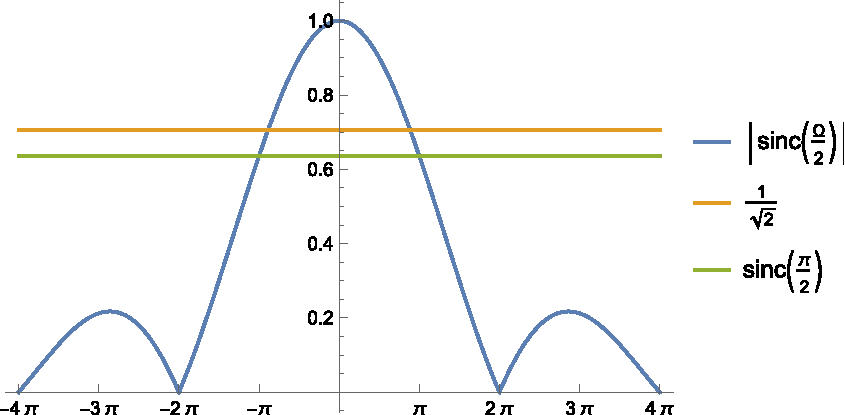
\includegraphics[keepaspectratio, scale=0.6]
                {\currfiledir/imgs/sinc-shaped_gain_distortion_with_ideal_DA.pdf}
                \caption{量子化誤差のないDA変換結果の sinc 状ゲイン歪み}
            \end{figure}
            上の図から、第1 Nyquist 領域の端 $-\pi, \pi$ で約 -3dB のゲイン低下が生じていることが解る。
            実は0次ホールドで出力する直前に、上手く設計された10タップ程度の FIR フィルタを掛けてこの影響を緩和し、下図のようなゲイン特性に変更できる。
            このフィルタは一般に 「inverse-sinc フィルタ」と呼ばれる。
            \begin{figure}[H]
                \centering
                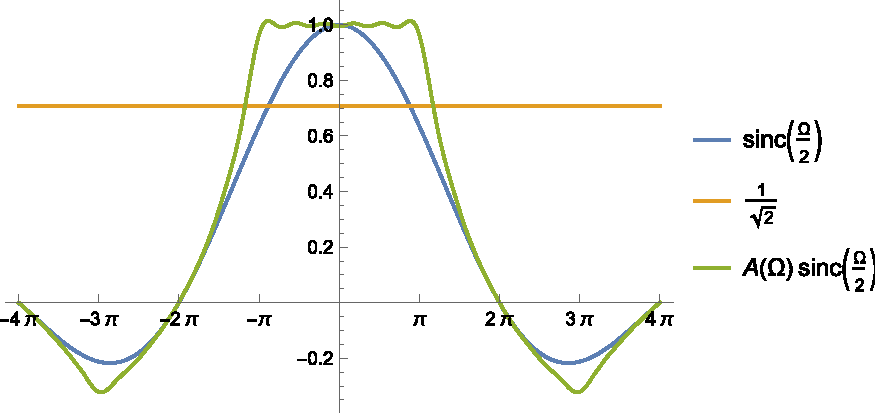
\includegraphics[keepaspectratio, scale=0.6]
                {\currfiledir/imgs/mitigated_distortion_with_inverse-sinc_filter.pdf}
                \caption{inverse-sinc フィルタによって緩和されたゲイン歪み(凡例の3つ目の曲線)}
                \label{inverse-sinc フィルタによって緩和されたゲイン歪み}
            \end{figure}
            inverse-sinc フィルタは $[-\pi, \pi]$ で sinc 状歪みの逆特性を近似するフィルタである。
            DA変換の対象とする信号は通常、サンプリング定理を念頭に置いてスペクトラムが $[-\pi,\pi]$ の領域に収まる信号であるから、上述の補正が十分に機能する。
            以下ではこのフィルタの設計方法の1つを述べる。
        \subsection{係数の導出}
            大雑把に言えば、フィルタ係数に対応する DTFT が $[-\pi,\pi]$ で $1/\sinc(\Omega/2)$ を近似するように最小二乗法で係数を決定する。
            \par
            フィルタ係数 $a:\integers\to\realNumbers$ は偶対称な実数値関数とし、非零の係数の個数を奇数とする。
            数式で述べれば $N\in\naturalNumbers,\;\forall n\in\integers\;a(-n) = a(n),\forall n>N\;a(n) = 0$ である。
            この制約条件が唯一の方法ではないだろうが、後に見るようにこれで十分な性能を得られる。
            \par
            $a$ の DTFT を $A$ とする。すなわち
            \[ A(\Omega) = \sum_{n=-N}^N a(n)\exp(-i\Omega n) = a(0) + 2\sum_{n=1}^N\cos(\Omega n) = \bm{v}(\Omega)^\top\bm{a} \]
            ここに $\bm{v}(\Omega) \coloneqq [1, 2\cos\Omega,\dots,2\cos N\Omega]^\top\in\realNumbers^{N+1},\;\bm{a} = [a(0),\dots,a(N)]^\top\in\realNumbers^{N+1}$ である。
            $[-\pi,\pi]$ で $A$ が $1/\sinc(\Omega/2)$ を近似するように次式を最小化する $a$ を求める。
            \[ \integrate{-\pi}{\pi}{\norm{A(\Omega) - 1/\sinc(\Omega/2)}_2^2}{}{\Omega} \tag{1} \]
            被積分関数の中身を展開すると次式を得る。
            \[ \norm{A(\Omega) - 1/\sinc(\Omega/2)}_2^2 = \bm{a}^\top\bm{v}(\Omega)\bm{v}(\Omega)^\top\bm{a} - \frac{2}{\sinc(\Omega/2)}\bm{v}(\Omega)^\top\bm{a} + 1/\sinc(\Omega/2)^2 \]
            これを式(1)に適用すると次式を得る。
            \[ (1) = \bm{a}^\top M\bm{a} - 2\bm{m}^\top\bm{a} + \integrate{-\pi}{\pi}{1/\sinc(\Omega/2)^2}{}{\Omega} \tag{2} \]
            ここに $M,\bm{m}$ は次式で定義される数である。
            \[ M \coloneqq \integrate{-\pi}{\pi}{\bm{v}(\Omega)\bm{v}(\Omega)^\top}{}{\Omega} = 2\pi\diag{1,2,2,\dots,2},\quad \bm{m} = \integrate{-\pi}{\pi}{\bm{v}(\Omega)^\top/\sinc(\Omega/2)}{}{\Omega} \]
            $\bm{m}$ は数値計算で求める。
            式(2)の中で $\bm{a}$ に依存しない項を無視すると、最小化すべき関数は次式である。
            \[ f_\text{cost}(\bm{a}) = \bm{a}^\top M\bm{a} - 2\bm{m}^\top\bm{a} \]
            これは狭義凸関数であり $(\nabla f)(\bm{a}) = 2(M\bm{a} - \bm{m})$ なので $f$ を最小化する $\bm{a}$ を $\bm{a}_\text{opt}$ は $M^{-1}\bm{m} = \diag{m_0,m_1 /2,\dots,m_N /2}/(2\pi)$ である。
            ここに $m_i\;(i=0,1,\dots,N)$ は $\bm{m}$ の第 $i$ 要素である。
        \subsection{数値例}
            $N=5$ のとき $\bm{a}_\text{opt} \approx [1.166240, -0.106996, 0.034475, -0.016454, 0.009530, -0.006189]^\top$ を得る。
            次の図はこの係数をプロットしたものである。
            \begin{figure}[H]
                \centering
                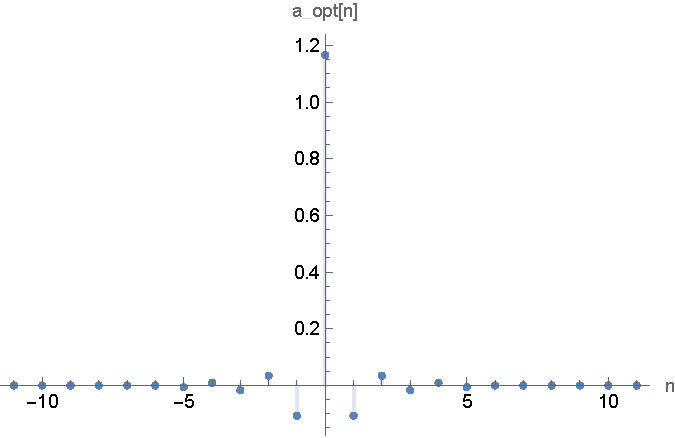
\includegraphics[keepaspectratio, scale=0.6]
                {\currfiledir/imgs/coeffs_of_inverse-sinc_filter.pdf}
                \caption{inverse-sinc フィルタの係数($N$=5)}
            \end{figure}
            次の図は、この係数に対応するフィルタのインパルス応答の DTFT と $1/\sinc(\Omega/2)$ を比較したものである。
            \begin{figure}[H]
                \centering
                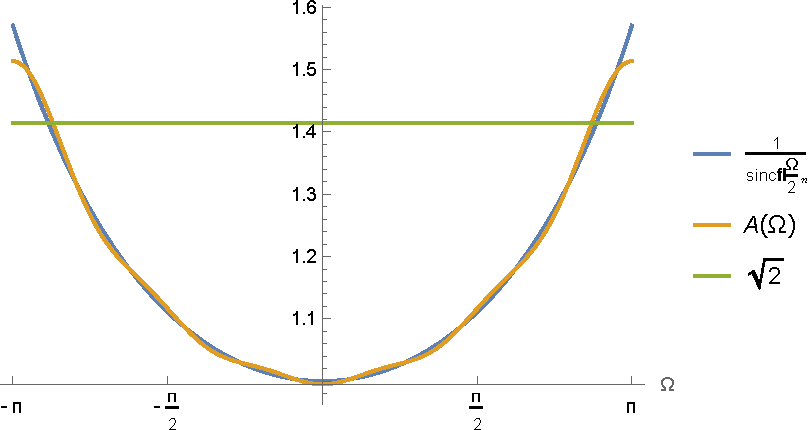
\includegraphics[keepaspectratio, scale=0.6]
                {\currfiledir/imgs/inverse-sinc_approximation.pdf}
                \caption{inverse-sinc フィルタのインパルス応答の DTFT}
            \end{figure}
            このフィルタを使ってゲイン歪みを緩和したのが先に挙げた図\ref{inverse-sinc フィルタによって緩和されたゲイン歪み}である。
    \section{0次ホールドされた正弦波の周波数特性}
        \label{0次ホールドされた正弦波の周波数特性}
        \subsection{背景}
            既に述べたように、信号処理や制御工学では実用上、入力と制御対象の間に0次ホールド回路と演算回路が挟まった形になる。
            技術書の中にはこれをステップ入力に対するラプラス変換の積分と時間遅れとして表してゲインや位相を考えているものもあるが、これは厳密には正しくない。
            なぜなら、0次ホールド回路に正弦波を入れた際、通過した信号は細かいステップの集まりであり、元の正弦波に近いものの、完全な正弦波ではないからである。
            「ゲイン」や「位相変化」を厳密に定義できない。
            厳密には、Fourier変換してスペクトラムについて考える必要がある。
            とはいえ、無限に続く減衰しない信号のFourier変換は通常の関数の意味では存在しないし(超関数になる)、現実の測定器は窓関数で時間制限した信号のFourier変換を近似的に計算している。
            そこで本記事では窓関数付きのFourier変換の結果ついて考察する。
        \subsection{導出}
            $f_0>0$とし、連続時間の複素正弦波信号$x:t\in\realNumbers\mapsto\exp(i 2\pi f_0 t)$を考える。
            サンプリング周期を$\Ts>0$とする。
            この周期で$x$を0次ホールドした信号を$\xd:t\in\realNumbers\mapsto x(\floor{t/\Ts}\Ts)$とする。
            次の図は$x$と$\xd$の実部を示したものである。
            \begin{figure}[H]
                \centering
                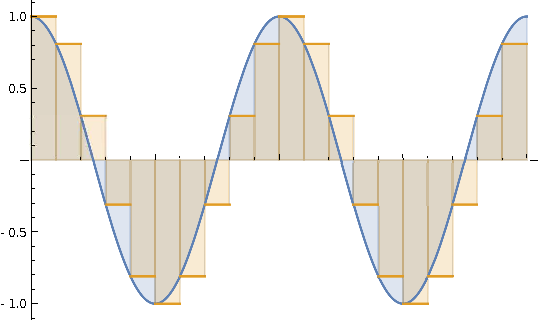
\includegraphics[keepaspectratio, scale=0.6]
                {\currfiledir/imgs/0-order-held-sinusoid.pdf}
                \caption{元の信号とその0次ホールド}
            \end{figure}
            上の図より、$\xd$の基本周波数成分(周波数成分に於ける$f_0$に対応する成分)が$x$のそれより遅れることが予想される。
            このことを矩形窓を通した、周波数表示されたFourier変換で考察する。
            $N\in\naturalNumbers$とし、窓の幅を$T=N\Ts$とする。
            窓の幅を$\Ts$の整数倍に選んでいるが、非整数倍の場合でも幅を十分に大きくとれば小数部分に対応する区間の積分の$1/T$倍は無視できるほど小さくなり、最も近い整数倍の幅を用いた結果と殆ど一致する。
            $x$の窓付きFourier変換を窓の幅で規格化したものは次式である。
            \[ X(f) = \frac{1}{T} \integrate{0}{T}{x(t)\exp(-i 2\pi f t)}{}{t} = \frac{1}{i 2\pi(f-f_0)T}\left(1-\exp\left(-i 2\pi(f-f_0)T\right)\right) \]
            $\xd$の窓付きFourier変換は次式である。
            \begin{align*}
                \Xd(f) &= \frac{1}{T}\integrate{0}{T}{\xd(t)\exp(-i 2\pi f t)}{}{t} = \frac{1}{T}\sum_{k=0}^{N-1}\integrate{k\Ts}{(k+1)\Ts}{\xd(t)\exp(-i 2\pi f t)}{}{t} \\
                &= \frac{1}{T}\sum_{k=0}^{N-1}\exp(i 2\pi f_0 k\Ts)\integrate{k\Ts}{(k+1)\Ts}{\exp(-i 2\pi f t)}{}{t} \\
                &= \frac{1}{T}\sum_{k=0}^{N-1}\exp(i 2\pi f_0 k\Ts)\frac{1}{i 2\pi f}\exp(-i 2\pi f k\Ts)\left(1-\exp(-i 2\pi f \Ts)\right) \\
                &= \frac{1-\exp(-i 2\pi f\Ts)}{i 2\pi f}\frac{1}{T}\underbrace{\sum_{k=0}^{N-1}\exp(i 2\pi(f_0-f)k\Ts)}_{\text{(A)}} \\
                &= \frac{1-\exp(-i 2\pi f\Ts)}{i 2\pi f}\frac{1}{N\Ts}\exp(i\pi(f_0-f)(N-1)\Ts)\frac{\sin\pi(f-f_0)N\Ts}{\sin\pi(f-f_0)\Ts}
            \end{align*}
            最後の式を導くために、(A)に等比数列の和の公式を適用し、分母・分子それぞれ$\sin$が生じるように複素指数関数を括り出して整理した。
            \par
            $\xd$中の、周波数が$f_0$である成分の振幅と位相を調べる。
            $f\to f_0$の極限に関して次式が成り立つ。
            \[ \lim_{f\to f_0} \Xd(f) = \frac{1-\exp(-i 2\pi f_0\Ts)}{i 2\pi f_0\Ts} \]
            これより、上式に相当する振幅と位相の変化が生じる。
            サンプリングが十分に高速、すなわち$f_0\Ts\ll 1$であるとき上式は1に近づくので、振幅と位相の変化は無くなってゆく。
            \par
            次に、高調波領域を調べる。
            $|\Xd(f)|$は$1/\Ts$周期関数と$1/|f|$の積であるので、$|f|<\Ts/2$の部分の縮小コピーが高周波領域に於いて$1/\Ts$毎に現れる。
            これが高調波成分である。
        \subsection{数値例}
            今、$f_0=10,\;\Ts=10^{-2},\;N=200$とする。
            $f=f_0$に於ける振幅と位相は$|\Xd(f_0)| \approx 0.9836,\quad \angle \Xd(f_0) \approx \ang{-18.00}$となる。
            次の図は$f_0$近傍でのパワースペクトル$X,\Xd$を示したものである。
            \begin{figure}[H]
                \centering
                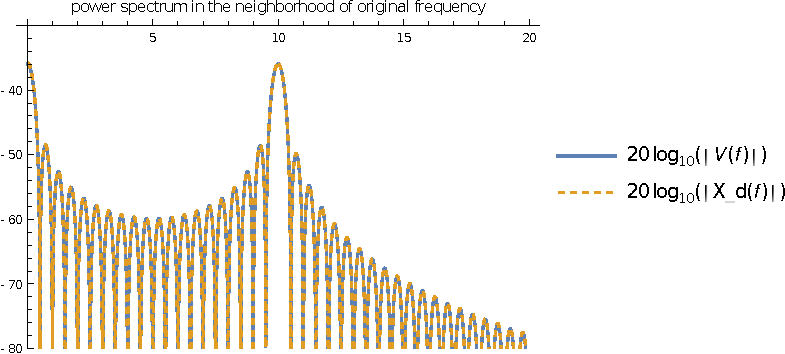
\includegraphics[keepaspectratio, scale=0.8]
                {\currfiledir/imgs/spectrum_in_the_neighborhood_of_original_frequency.pdf}
                \caption{元の周波数の近傍でのパワースペクトル}
            \end{figure}
            低周波領域では両者が良く一致していることがわかる。
            \par
            次に高調波を見る。
            次の図はサンプリング周波数の3倍の範囲まで$X,\Xd$を示したものである。
            \begin{figure}[H]
                \centering
                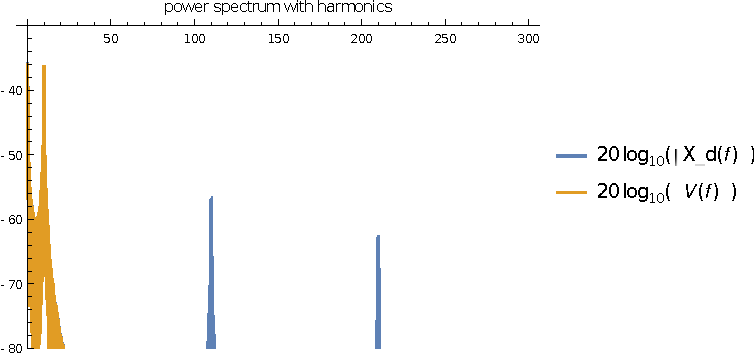
\includegraphics[keepaspectratio, scale=0.8]
                {\currfiledir/imgs/power_spectrum_with_harmonics.pdf}
                \caption{高調波を含むパワースペクトル}
            \end{figure}
            サンプリング周波数の整数倍の位置に高調波が生じていることが判る。
            \par
            この数値例を計算したMathematicaノートブックおよびMATLABスクリプトは下記のファイル名で保存されている。
            Gitリポジトリ内でファイル名検索すれば発見できるであろう。
            \begin{itemize}
                \item \href{\currfiledir/spectrum_of_zero-order-held-sine-wave.nb}{spectrum\_of\_zero\-order\-held\-sine\-wave.nb}
                \item \href{\currfiledir/spectrum_of_zero_order_held_sine_wave.m}{spectrum\_of\_zero\_order\_held\_sine\_wave.m}
            \end{itemize}
    \section{入力に0次ホールド機構を加えた連続時間システムのz変換}
        \subsection{背景}
            実用上、物理系をディジタル計算機で制御するために、連続系である制御対象と入力の間に「AD変換器」(0次ホールド回路+量子化器),「演算回路」,「DA変換器」(0次ホールド回路)が追加される。
            本節では、連続時間システムの入力に0次ホールド機構を追加したときのシステムの出力のうち、サンプリング時間の整数倍の時点に於いて出力が厳密に一致する離散時間システムのz変換を導出する。
        \subsection{主張}
            \renewcommand{\uH}{u_\text{H}}
            \newcommand{\ud}{u_\text{d}}
            \newcommand{\udd}{u_\text{dd}}
            \newcommand{\yd}{y_\text{d}}
            \newcommand{\ydd}{y_\text{dd}}
            \newcommand{\hd}{h_\text{d}}
            \newcommand{\hdd}{h_\text{dd}}
            \newcommand{\Ud}{U_\text{d}}
            \newcommand{\Udd}{U_\text{dd}}
            \newcommand{\Hd}{H_\text{d}}
            \newcommand{\Hdd}{H_\text{dd}}
            \newcommand{\Yd}{Y_\text{d}}
            \newcommand{\Ydd}{Y_\text{dd}}
            連続時間システムのインパルス応答を$h:\realNumbers\to\complexNumbers$とし、そのラプラス変換を$H:\complexNumbers\to\complexNumbers$とする。
            但しシステムは因果的である、すなわち$h(t)=0\;(t<0)$とする。
            入力信号をサンプリング周期$\Ts>0$で0次ホールドして与えるときの出力を$\yd:\realNumbers\to\complexNumbers$とする。
            このとき、システムのz領域の伝達関数は$(1-z^{-1})\Hdd(z)$となる。
            ここに$\Hdd(z)$は$H(s)/s$の逆ラプラス変換を周期$\Ts$でサンプリングして得られる離散時間信号のz変換である。
            つまり、このz領域の伝達関数の出力は$\Ts$の整数倍の時刻で連続時間システムの出力$\yd$と厳密に一致する。
            \begin{figure}[H]
                \centering
                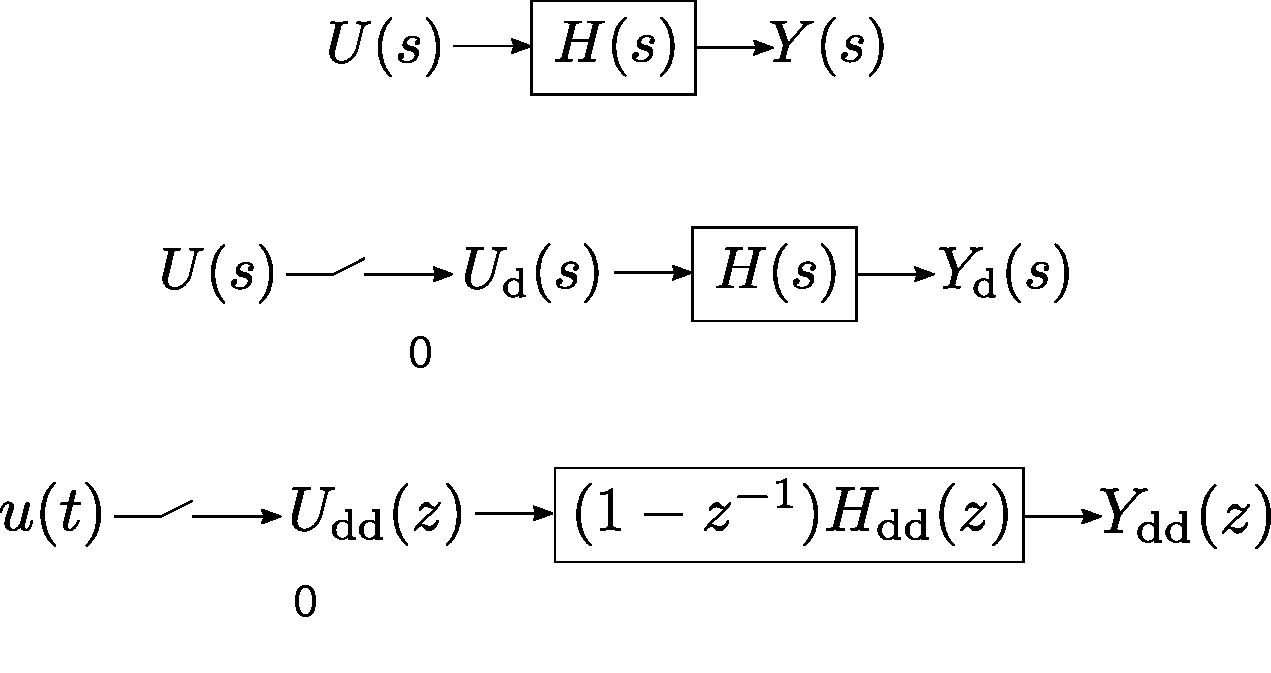
\includegraphics[keepaspectratio, scale=0.4]
                {\currfiledir/imgs/z-transform_with_0-order-hold_input.pdf}
                \caption{連続時間系と、入力に0次ホールドを付加した系}
            \end{figure}
        \subsection{導出}
            連続時間システムへの入力を$u:\realNumbers\to\complexNumbers$とする。
            但し$u(t)=0\;(t<0)$とする。
            周期$\Ts$で0次ホールドされた入力信号を$\ud:t\in\realNumbers\to u(\floor{t/\Ts}\Ts)$とする。
            Heavisideの単位ステップ関数を$\uH$とすると$\ud$は次式で表せる。
            \[ \ud(t) = \sum_{k=0}^\infty u(k\Ts)\left(\uH(t-k\Ts) - \uH(t-(k+1)\Ts)\right) \]
            これのラプラス変換を$U_\text{d}$とすると次式で表される。
            \[ \Ud(s) = \sum_{k=0}^\infty u(k\Ts)\NapierE^{-k\Ts s}\frac{1-\NapierE^{-\Ts s}}{s} \]
            これに対する出力$\yd$のラプラス変換を$\Yd$とすると、次式である。
            \begin{align*}
                \Yd(s) &= \sum_{k=0}^\infty u(k\Ts)\NapierE^{-k\Ts s}\frac{1-\NapierE^{-\Ts s}}{s}H(s) = \sum_{k=0}^\infty u(k\Ts)\NapierE^{-k\Ts s}\left(1-\NapierE^{-\Ts s}\right)\Hd(s) \\
                &\phantom{=} \text{where} \quad \Hd(s) \coloneqq H(s)/s
            \end{align*}
            $\Hd(s)$の逆ラプラス変換を$\hd$とすると、$\yd$は次式である。
            \[ \yd(t) = \sum_{k=0}^\infty u(k\Ts)(\hd(t-k\Ts)-\hd(t-(k+1)\Ts)) \]
            離散時間信号$\hdd,\ydd$を$\hdd:n\in\integers\mapsto \hd(n\Ts),\ydd:n\in\integers\mapsto \yd(n\Ts)$とすると$\ydd$は次式である。
            \begin{align*}
                \ydd(n) &= \yd(n\Ts) = \sum_{k=0}^\infty u(k\Ts)(\hd((n-k)\Ts)-\hd((n-k-1)\Ts)) \\
                &= \sum_{k=0}^\infty u(k\Ts)(\hdd(n-k)-\hdd(n-k-1))
            \end{align*}
            離散時間信号$\udd$を$\udd:n\in\integers\mapsto\ud(n\Ts)$で定義する。
            $\udd,\hdd,\ydd$のz変換をそれぞれ$\Udd,\Hdd,\Ydd$とすると次式を得る。
            \begin{align*}
                \Ydd(z) &= \sum_{n=0}^\infty \ydd(n) z^{-n} = \sum_{k=0}^\infty \ud(k\Ts) \sum_{n=0}^\infty ((\hdd(n-k)-\hdd(n-k-1))) z^{-n} \\
                &= \sum_{k=0}^\infty \ud(k\Ts)\left[z^{-k}\sum_{n=0}^\infty \hdd(n-k)z^{-(n-k)} - z^{-k-1}\sum_{n=0}^\infty \hdd(n-k-1)z^{-(n-k-1)}\right] \\
                &= \sum_{k=0}^\infty \ud(k\Ts)\left[z^{-k}\sum_{n=k}^\infty \hdd(n-k)z^{-(n-k)} - z^{-k-1}\sum_{n=k+1}^\infty \hdd(n-k-1)z^{-(n-k-1)}\right] \\
                &= \left(\sum_{k=0}^\infty \ud(k\Ts)z^{-k}\right)(1-z^{-1})\Hdd(z) = \Udd(z)(1-z^{-1})\Hdd(z)
            \end{align*}
